\documentclass{article}\usepackage[]{graphicx}\usepackage[]{xcolor}
% maxwidth is the original width if it is less than linewidth
% otherwise use linewidth (to make sure the graphics do not exceed the margin)
\makeatletter
\def\maxwidth{ %
  \ifdim\Gin@nat@width>\linewidth
    \linewidth
  \else
    \Gin@nat@width
  \fi
}
\makeatother

\definecolor{fgcolor}{rgb}{0.345, 0.345, 0.345}
\newcommand{\hlnum}[1]{\textcolor[rgb]{0.686,0.059,0.569}{#1}}%
\newcommand{\hlsng}[1]{\textcolor[rgb]{0.192,0.494,0.8}{#1}}%
\newcommand{\hlcom}[1]{\textcolor[rgb]{0.678,0.584,0.686}{\textit{#1}}}%
\newcommand{\hlopt}[1]{\textcolor[rgb]{0,0,0}{#1}}%
\newcommand{\hldef}[1]{\textcolor[rgb]{0.345,0.345,0.345}{#1}}%
\newcommand{\hlkwa}[1]{\textcolor[rgb]{0.161,0.373,0.58}{\textbf{#1}}}%
\newcommand{\hlkwb}[1]{\textcolor[rgb]{0.69,0.353,0.396}{#1}}%
\newcommand{\hlkwc}[1]{\textcolor[rgb]{0.333,0.667,0.333}{#1}}%
\newcommand{\hlkwd}[1]{\textcolor[rgb]{0.737,0.353,0.396}{\textbf{#1}}}%
\let\hlipl\hlkwb

\usepackage{framed}
\makeatletter
\newenvironment{kframe}{%
 \def\at@end@of@kframe{}%
 \ifinner\ifhmode%
  \def\at@end@of@kframe{\end{minipage}}%
  \begin{minipage}{\columnwidth}%
 \fi\fi%
 \def\FrameCommand##1{\hskip\@totalleftmargin \hskip-\fboxsep
 \colorbox{shadecolor}{##1}\hskip-\fboxsep
     % There is no \\@totalrightmargin, so:
     \hskip-\linewidth \hskip-\@totalleftmargin \hskip\columnwidth}%
 \MakeFramed {\advance\hsize-\width
   \@totalleftmargin\z@ \linewidth\hsize
   \@setminipage}}%
 {\par\unskip\endMakeFramed%
 \at@end@of@kframe}
\makeatother

\definecolor{shadecolor}{rgb}{.97, .97, .97}
\definecolor{messagecolor}{rgb}{0, 0, 0}
\definecolor{warningcolor}{rgb}{1, 0, 1}
\definecolor{errorcolor}{rgb}{1, 0, 0}
\newenvironment{knitrout}{}{} % an empty environment to be redefined in TeX

\usepackage{alltt}
\usepackage{amsmath} %This allows me to use the align functionality.
                     %If you find yourself trying to replicate
                     %something you found online, ensure you're
                     %loading the necessary packages!
\usepackage{amsfonts}%Math font
\usepackage{graphicx}%For including graphics
\usepackage{hyperref}%For Hyperlinks
\usepackage[shortlabels]{enumitem}% For enumerated lists with labels specified
                                  % We had to run tlmgr_install("enumitem") in R
\hypersetup{colorlinks = true,citecolor=black} %set citations to have black (not green) color
\usepackage{natbib}        %For the bibliography
\setlength{\bibsep}{0pt plus 0.3ex}
\bibliographystyle{apalike}%For the bibliography
\usepackage[margin=0.50in]{geometry}
\usepackage{float}
\usepackage{multicol}

%fix for figures
\usepackage{caption}
\newenvironment{Figure}
  {\par\medskip\noindent\minipage{\linewidth}}
  {\endminipage\par\medskip}
\IfFileExists{upquote.sty}{\usepackage{upquote}}{}
\begin{document}

\vspace{-1in}
\title{Lab 10 -- MATH 240 -- Computational Statistics}

\author{
  Ben Horner \\
  Colgate University  \\
  Math Department  \\
  {\tt bhorner@colgate.edu}
}

\date{}

\maketitle

\begin{multicols}{2}
%\raggedcolumns % If your spacing gets messed up try uncommenting 
                % this line
\begin{abstract}
In many polls and other research, the margin of error is essential to understanding and contextualizing the results. Gallup polls claims that for a sample sie of 1000, selected with careful procedures, their results are likely to be accurate within a margin of error of $\pm 4\%$, and that doubling their sample size will only effectively half their margin of error. Examining these claims illustrate that with their published data, they are indeed accurate within $\pm 4\%$, and that doubling the sample size actually reduces the margin of error by less than half. 
\end{abstract}

\noindent \textbf{Keywords:} Resampling; margin of error; sampling distribution; sample proportion

\section{Introduction}
Gallup polls is high profile polling, analysis, and consulting organization which often tries to track the opinions of Americans. To give further detail on their methodology, Gallup polls published a document called \emph{``How Are Polls Conducted?"} that describes how Gallup selects which people to include among other details. Towards the end of their document, they mention how using a sample of 1000 adults \emph{``derived using careflu random selection procedures"}, their results are \emph{``highly likely"} to be accurate within a $\pm 4\%$ margin of error. However, they also claim that increasing the sample size to 2000 reduces the margin of error to within $\pm 2\%$. 

To examine the veracity of these statements, we reexamine and recalculate the margin of error in their February 3\-16, 2025 poll of 1004 adults from their representative sample which revealed that $39\%$ of respondents were satisfied with the position of the United States in the world today, compared to $59\%$ who were dissatisfied ($2\%$ had no opinion). Gallup reported the same $\pm 4\%$ margin of error. 




\section{Methods}
Often, statisticians and quantitative researchers will report a margin of error that provides $95\%$ confidence. We will use the same confidence interval when examining the Gallup poll data.

\subsection{Basic Simluation}
Before delving into the real data, we want to conduct a basic simulation study which assumes the true probability that someone is satisfied with the position of the United States in the world today is $0.39$. After using \texttt{rbinom()} to generate 10k polls of the same 1004 person sample size, we can calculate the range of the middle $95\%$ of the resulting sampling distribution. Additionally, we can approximate the margin of error by halving that range to compare it to the $4\%$ reported by Gallup.

We also want to address Gallup's claims that doubling their sample size to around 2000 will resultingly half their margin of error from $4$ to $2\%$. This can be done by simply repeating the same basic simulation and adjusting the sample size to 2008 (double the original 1004) and repeating the same calculations.

\subsection{Resampling}
After simulating what the sampling distribution would look like after making an assumption about the actual population proportion, we examine how resampling can be used to approximate the sampling distribution for \emph{p}. After importing the data from the original Gallup survey, we resampled 10k times to reflect our simulation. The range of the middle $95\%$ and margin of error are calculated the same as with the basic simulation. 

\subsection{Simulation over $n$ and $p$}
To provide better guidance for Gallup readers, simulating over sample sizes $n$ in \{100, 110, 130, ..., 3000\} and $p$ in \{0.01, 0.02, ..., 0.99\} can provide us with a better understanding of how the margin of error changes with polls. 

\subsection{Actual Margin of Error}
Finally, as we have been estimating the margin of error as half the range of the middle $95\%$, we now compute the Wilson margin of error for the same set of $n$ and $p$ values. We use the \texttt{geom\_raster()} function to visualize these two simulations over $n$ and $p$.

\section{Results}
When we conduct the basic simulation study, assuming the population level values, the resulting sampling proportions follow a normal distribution.
\begin{knitrout}\scriptsize
\definecolor{shadecolor}{rgb}{0.969, 0.969, 0.969}\color{fgcolor}
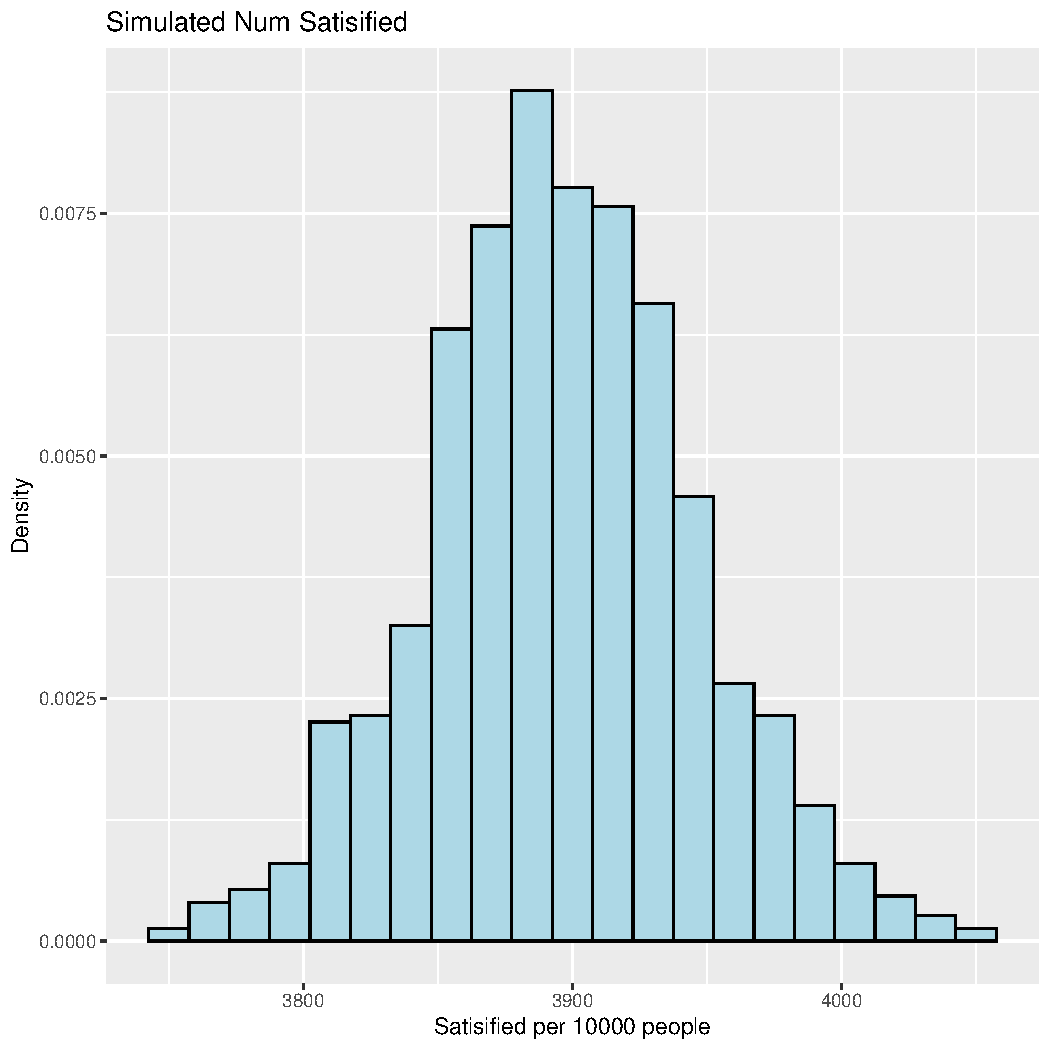
\includegraphics[width=\maxwidth]{figure/unnamed-chunk-1-1} 
\end{knitrout}
The resulting middle $95\%$ of the data falls in range 192.925 with the estimated margin of error of 96.4625 people satisfied. Doubling the sample size reduces the middle range to 184.825 and the margin of error to 92.4125 people satisfied. 

Using the true data and the resampling method also outputs a normally distributed sampling distribution.
\begin{knitrout}\scriptsize
\definecolor{shadecolor}{rgb}{0.969, 0.969, 0.969}\color{fgcolor}\begin{kframe}
\begin{verbatim}
## [1] 392
\end{verbatim}
\end{kframe}
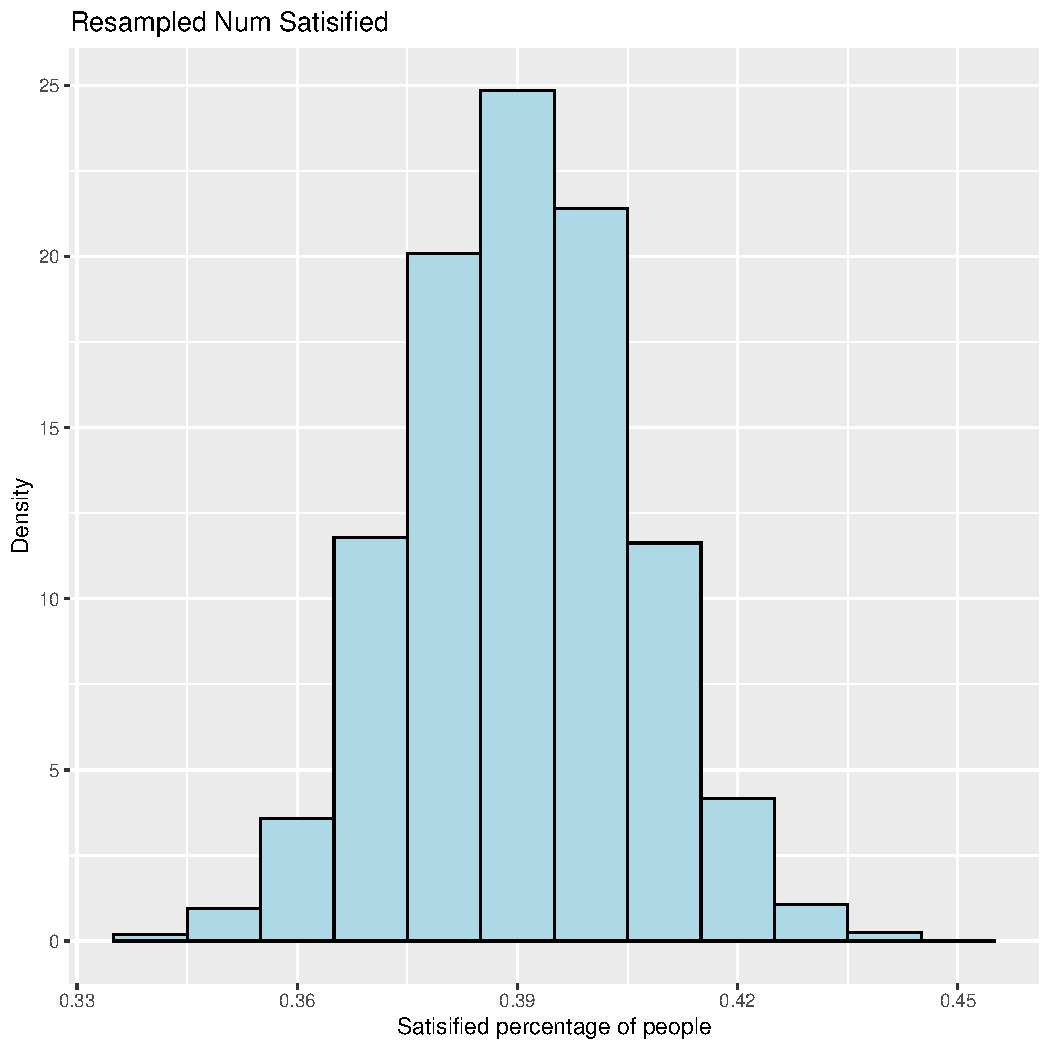
\includegraphics[width=\maxwidth]{figure/unnamed-chunk-2-1} 
\end{knitrout}
In this case, our margin of error as a percentage is $3.04\%$, which is within Gallup's claims that they are accurate withing $\pm 4\%$. 


\section{Discussion}
As Gallup claims that their data is accurate to within $\pm 4\%$, we found that via simulating and reusing their data, this claim is true. However, when we doubled the sample size in the simulated data, as we cannot double their actual data, the margin of error did not half as they state it does. 

%%%%%%%%%%%%%%%%%%%%%%%%%%%%%%%%%%%%%%%%%%%%%%%%%%%%%%%%%%%%%%%%%%%%%%%%%%%%%%%%
% Bibliography
%%%%%%%%%%%%%%%%%%%%%%%%%%%%%%%%%%%%%%%%%%%%%%%%%%%%%%%%%%%%%%%%%%%%%%%%%%%%%%%%
\vspace{2em}



\begin{tiny}
\bibliography{bib}
\end{tiny}
\end{multicols}


\end{document}
